\chapter{2D case}

% {{{1 PROBLEM
\section{Problem}

In this part, we will focus on a 2D point cloud and we will use for the energy
the area of the $ r $-offset of a point cloud $ X $: the union of the balls
centered on the point cloud with radius $r$. We will also test other types of
energies like the perimeter of the boundary, and weighted ones...

Firstly, we will show how to compute the area of the union of balls.
Then, we will run different experiments to verify that the gradient of
the union of balls is proportional to the mean curvature of the underlying
curve. Finally, we will run our programs on different point clouds with
different parameters to show that it can simulate discrete mean curvature flows.

% {{{1 AREA OF A UNION OF BALLS
\section{Area of a union of balls}

For this part, we will need the definition of the Voronoi diagram of set of
points:

\begin{definition}
    Given a set of points $ P \in E $, we define the Voronoi cell of $ p \in P $
    denoted by $ V(p, P) $:
    $$ V(p, P) = \{ q \in E,~ \forall p' \neq p \in P,~|| p  - q || \leq || p' -
    q || \} $$
    In short, the Voronoi cell of $ p $ is composed of all the points which are
    closer to $ p $ than to any other points in $ P $.

    Then, the Voronoi diagram of $ P $ is composed of all the Voronoi cells of $
    p \in P $. It is a partition of the space $ E $.
\end{definition}

For example, the figure \ref{fig:voronoi-diagram-2d} is an example of a Voronoi
diagram.

\begin{figure}[h]
    \centering
    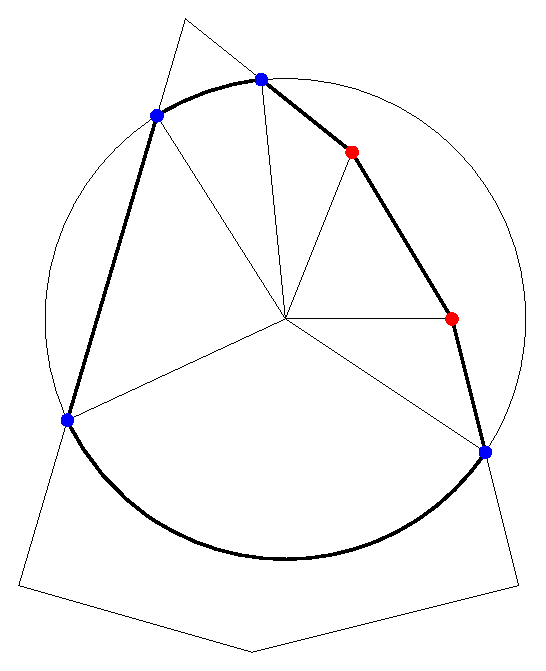
\includegraphics[scale=0.4]{voronoi-diagram-2d}
    \caption{Points are in black and the boundary of the Voronoi cells are in
        red}
    \label{fig:voronoi-diagram-2d}
\end{figure}

Now, we can say that, because the Voronoi diagram is a partition, we have, for a
point cloud $ P $ :

$$ Area(P^r) = Area \left( \bigcup_p B(p, r) \right) = \sum_p Area(V(p, P) \cap B(p, r)) $$

In order to compute this quantity, we need to know how to estimate the area of the
intersection of a ball and a Voronoi cell. In 2D, the boundary of the
intersection between a Voronoi cell and a ball is composed of segments and
circular arcs.

The figures \ref{fig:inter_voronoi_ball_2d} illustrate the different cases for
the intersection of a Voronoi cell and a ball in 2D.

\begin{figure}[h]
    \centering
    \begin{minipage}{0.32\linewidth}
        \centering
        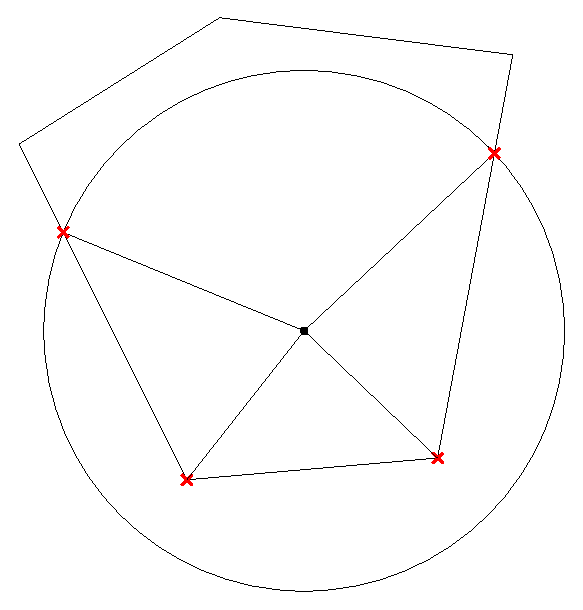
\includegraphics[scale=0.4]{2d/inter_voronoi_ball_2d}
        \subcaption{General case}
        \label{fig:inter_voronoi_ball_2d:a}
    \end{minipage}
    \begin{minipage}{0.32\linewidth}
        \centering
        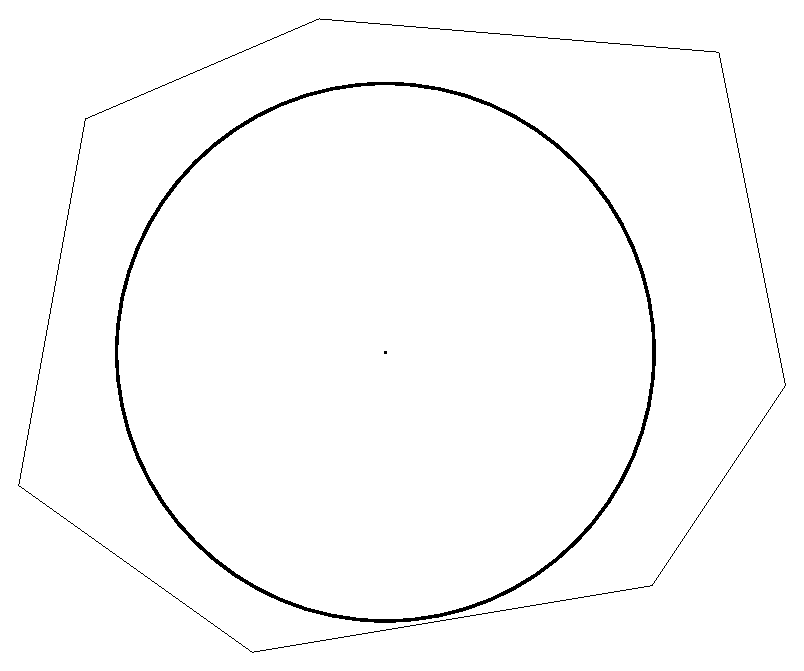
\includegraphics[scale=0.4]{2d/inter_voronoi_ball_2d_no_inter}
        \subcaption{No intersections}
        \label{fig:inter_voronoi_ball_2d:b}
    \end{minipage}
    \begin{minipage}{0.32\linewidth}
        \centering
        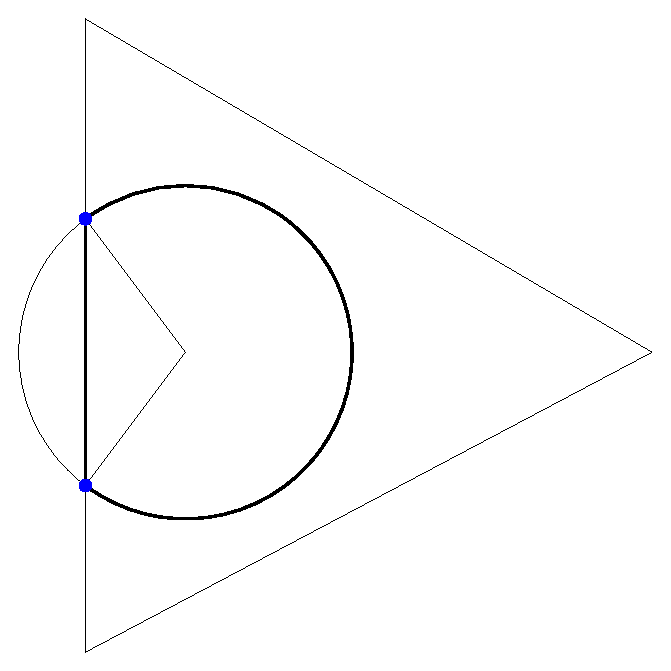
\includegraphics[scale=0.4]{2d/inter_voronoi_ball_2d_2_inter}
        \subcaption{2 intersections}
        \label{fig:inter_voronoi_ball_2d:c}
    \end{minipage}

   \caption{Different cases for the intersection between a Voronoi cell and a sphere}
   \label{fig:inter_voronoi_ball_2d}
\end{figure}

We use \texttt{CGAL} to compute the Delaunay triangulation of our point set: it
is the dual graph of the Voronoi diagram. A triangle in the Delaunay
triangulation corresponds to a vertex in the Voronoi diagram, an edge
corresponds to an edge, a vertex corresponds to a face...

Given this triangulation, we can compute the vertices composing the boundary of
the  Voronoi cell (in bold in the figures \ref{fig:inter_voronoi_ball_2d}) of a
point by doing the following:
\begin{enumerate}
    \item Access the neighbouring faces of a vertex using the
        \texttt{incident\_faces} method.
    \item Compute the Voronoi vertices (circumcenters) of these faces using the
        \texttt{dual} method.
\end{enumerate}

There are two types of points on the boundary: some are Voronoi vertices (in
red) and some are intersections of Voronoi edges and circles (in blue). We will
refer to the red points as the interior points.
To each of the points, we attach a boolean saying whether the point is an
interior one or an intersection one. We also attach to each point its
corresponding Voronoi edge.

Then, we loop over the boundary of the Voronoi cell of $ v $, for any edge $ e =
pq $. Depending on whether the points $ p $ and $ q $ are interior or not, the
contribution to the area of $ e $ will be different:
\begin{itemize}
    \item if $ p $ and $ q $ are interior points, we add the triangle $ pvq $.
    \item if $ p $ or $ q $ is interior point, we add the triangle $ pvq $.
    \item if $ p $ and $ q $ are intersection points, then if they belong to the
        same Voronoi edge, we add the triangle $ pvq $. If not, we add the
        angular sector $ \vec{vp}, \vec{vq} $.
\end{itemize}

Some special cases need to be handled:
\begin{itemize}
    \item the boundary of the Voronoi cell is entirely outside the ball, then we
        add $ \pi r^2 $ to the area of the union (see
        \ref{fig:inter_voronoi_ball_2d:b}).
    \item the boundary consists of two intersection points $ p $ and $ q $, then
        we add the triangle $ pvq $ and the angular sector $ \vec{vp}, \vec{vq}
        $ (see \ref{fig:inter_voronoi_ball_2d:c}).
    \item there is only one point on the boundary (can happen if adjacent balls
        are tangential), then we add $ \pi r^2 $.
\end{itemize}

This algorithm allows us to compute exactly the area of a union of balls.

We use the same techniques for computing the perimeter of the boundary of the
intersection except that if there are no intersection then the perimeter is null
and instead of adding triangles areas or angular sectors, we add lengths of
circular arcs.

% {{{1 IMPLEMENTATION DETAILS
\section{Implementation details}

For the implementation, we used different libraries: \texttt{CGAL} which is a
C++ library that offers all the basic geometric types (point, vector, line,
plane..), data structures and algorithms (triangulations...). We also used
\texttt{Eigen} which is a C++ linear algebra library which provides types such
as vector, matrix and manipulation operations. We used \texttt{Qt} for the GUI
programming.

The main difficulty here was to compute the intersection between a Voronoi cell
and a circle. The Voronoi cell is computed using its dual graph: the Delaunay
triangulation. The intersection procedure was described previously.

We also used the automatic differentiation technique (see the appendix
\ref{appendix:ad}): it allowed us to only care about the computation of the area
and not its gradient.

% {{{1 GRADIENT
\section{Gradient}

In this section, we will study the gradient of the area of union of balls, the
perimeter of the boundary

We used the automatic differentiation technique described in the appendix
\ref{appendix:ad} to compute the gradient of the previously computed area.

See the figures \ref{fig:gradients_area_2d} for a few examples of such gradients
for different input point sets.

\begin{figure}[h]
    \centering

    \begin{minipage}{0.8\linewidth}
        \centering
        \includegraphics[scale=0.3]{2d/area/ellipse-100-01-15}
        \includegraphics[scale=0.3]{2d/area/ellipse-100-01-15-gradients}
        \subcaption{Gradients of the area for 100 samples on an ellipse}
        \label{fig:gradients_area_2d_ellipse}
    \end{minipage}

    \begin{minipage}{0.8\linewidth}
        \centering
        \includegraphics[scale=0.32]{2d/area/circle-100-01-15}
        \includegraphics[scale=0.32]{2d/area/circle-100-01-15-gradients}
        \subcaption{Gradients of the area for 100 samples on a circle}
        \label{fig:gradients_area_2d_circle}
    \end{minipage}

    \begin{minipage}{0.8\linewidth}
        \centering
        \includegraphics[scale=0.32]{2d/area/square-40-001-100}
        \includegraphics[scale=0.32]{2d/area/square-40-001-100-gradients}
        \subcaption{Gradients of the area for 40 samples on a square}
        \label{fig:gradients_area_2d_square}
    \end{minipage}

    \caption{Input point set / Computed gradients of the area}
    \label{fig:gradients_area_2d}
\end{figure}

We did the same thing using the gradient of the perimeter of the boundary on the
same point clouds (see the figures \ref{fig:gradients_perimeter_2d}).

\begin{figure}[h]
    \centering

    \begin{minipage}{0.8\linewidth}
        \centering
        \includegraphics[scale=0.3]{2d/perimeter/ellipse-100-01-15}
        \includegraphics[scale=0.3]{2d/perimeter/ellipse-100-01-15-gradients}
        \subcaption{Gradients of the perimeter for 100 samples on an ellipse}
        \label{fig:gradients_perimeter_2d_ellipse}
    \end{minipage}

    \begin{minipage}{0.8\linewidth}
        \centering
        \includegraphics[scale=0.32]{2d/perimeter/circle-100-01-15}
        \includegraphics[scale=0.32]{2d/perimeter/circle-100-01-15-gradients}
        \subcaption{Gradients of the perimeter for 100 samples on a circle}
        \label{fig:gradients_perimeter_2d_circle}
    \end{minipage}

    \begin{minipage}{0.8\linewidth}
        \centering
        \includegraphics[scale=0.32]{2d/perimeter/square-40-001-100}
        \includegraphics[scale=0.32]{2d/perimeter/square-40-001-100-gradients}
        \subcaption{Gradients of the perimeter for 40 samples on a square}
        \label{fig:gradients_perimeter_2d_square}
    \end{minipage}

    \caption{Input point set / Computed gradients of the perimeter}
    \label{fig:gradients_perimeter_2d}
\end{figure}

In the previous screenshots, we can see that the gradients are (if the radius of
the balls are big enough and if the sampling is sufficiently uniform) in the
same direction as the normals to the underlying surface. Also, the norm of
these gradients is related to the mean curvature of the approximated surface
(see proposition the proposition \ref{prop:gradient-mean-curvature}).

% {{{1 MEAN CURVATURE ESTIMATION
\section{Mean curvature estimation}

We can use the previous results to estimate mean curvature on a point set using
the norm of the gradients of the area of the union of balls.

We run our tests on a sampled ellipse whose major and minor axes are $ a $ and $
b $. We can parametrize this ellipse by :
$$
\begin{cases}
    x(t) &= a \cos (t) \\
    y(t) &= b \sin (t)
\end{cases}
\text{ for t } \in [ 0, 2\pi ]
$$

We recall the formula for computing the curvature of a parametrized curve:
$$ \kappa(t) = \frac{x'(t) y''(t) - y'(t) x''(t)}{(x'^2(t) +
    y'^2(t))^{\frac{3}{2}} } $$

For an ellipse, we obtain:
$$ \kappa(t) = \frac{ab}{(a^2 \cos^2(t) + b^2 \sin^2(t))^{\frac{3}{2}} } $$

We compare this for $ t = \frac{2 k \pi}{N} $ for $ k = 0 \ldots N - 1 $ with
the computed ones where $ N $ is the number of samples.

Figures \ref{fig:2d-curvature-ellipse-area} and \ref{fig:2d-curvature-ellipse-perimeter}
represent the computed gradients mapped to a colour ramp (from green to red), we
see that the gradients are more important where the curvature is higher and are
collinear to the outward normals.

\begin{figure}[h]
    \centering

    \includegraphics[scale=0.3]{2d/area/curvature-ellipse-200-15}
    \caption{Computed curvatures on an ellipse using gradients of the area with $ r = 15 $}
    \label{fig:2d-curvature-ellipse-area}

    \includegraphics[scale=0.3]{2d/perimeter/curvature-ellipse-200-15}
    \caption{Computed curvatures on an ellipse using gradients of the perimeter with $ r = 15 $}
    \label{fig:2d-curvature-ellipse-perimeter}
\end{figure}

% TODO: pictures

Now, we study the absolute difference between the computed and expected
curvatures for different choices of gradients (area, perimeter of the boundary,
weighted...), see the figures \ref{fig:2d-curvature-error-ellipse-area} and
\ref{fig:2d-curvature-error-ellipse-perimeter}.

\begin{figure}[h]
    \centering

    \includegraphics[scale=0.3]{2d/area/curvature-error-ellipse-200-05}
    \caption{Error between the curvatures on an ellipse using gradients of the area with $ r = 0.5 $}
    \label{fig:2d-curvature-error-ellipse-area}

    \includegraphics[scale=0.3]{2d/perimeter/curvature-error-ellipse-200-05}
    \caption{Error between the curvatures on an ellipse using gradients of the perimeter with $ r = 0.5 $}
    \label{fig:2d-curvature-error-ellipse-perimeter}
\end{figure}

% {{{1 DISCRETE MEAN CURVATURE FLOW
\section{Discrete Mean Curvature Flow}

Now, we will be interested in approximating the continuous mean curvature flow
by applying a gradient descent algorithm in order to minimize a functional $ E
$.

This gradient descent will be done using a constant timestep (Euler explicit
scheme).

We will also be interested in weighted versions of functionals: we can weight
the gradient of the area by the perimeter of the visible part (the circular arcs
composing the intersection of the Voronoi cell and the ball) of the restricted
region. But by doing that, we can divide by $ 0 $ so we need to choose a small
time step in order to avoid the case where a point does not see anything.

% TODO

We did some experiments to validate our results: we first compared the two
gradient flows (area and perimeter of the boundary) to a set of points uniformly
sampled on an ellipse: figures \ref{fig:ellipse_area_flow} and
\ref{fig:ellipse_perimeter_flow}.

% TODO: ajouter convergence vers cercle
\begin{figure}[h]
    \centering

    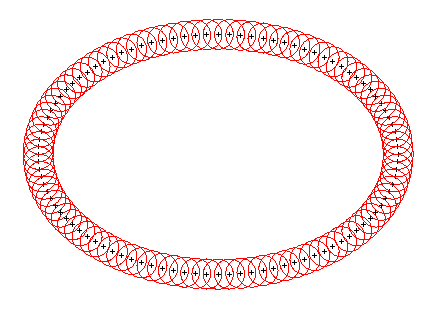
\includegraphics[scale=0.3]{2d/ellipse-balls-15}
    \subcaption{Minkowski sum of an ellipse and balls of radius $ 15 $}

    \includegraphics[scale=0.3]{2d/area/ellipse-100-01-15}
    \includegraphics[scale=0.3]{2d/area/ellipse-100-01-15-100}
    \subcaption{Area flow of an ellipse: 0 / 100 iterations with a timestep of $ 0.1 $}
    \label{fig:ellipse_area_flow}

    \includegraphics[scale=0.3]{2d/perimeter/ellipse-100-01-15}
    \includegraphics[scale=0.3]{2d/perimeter/ellipse-100-01-15-100}
    \subcaption{Perimeter flow of an ellipse: 0 / 100 iterations with a timestep of $ 0.5 $}
    \label{fig:ellipse_perimeter_flow}

    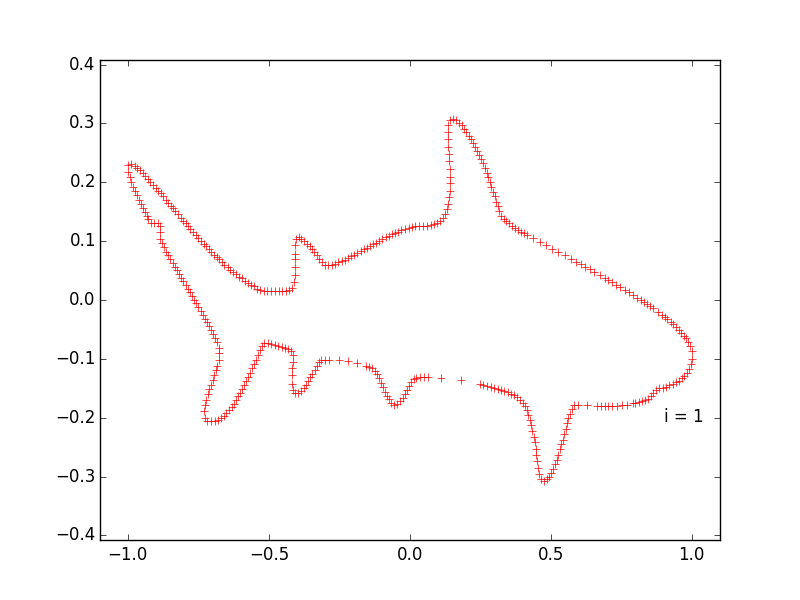
\includegraphics[scale=0.22]{2d/perimeter/shark-0}
    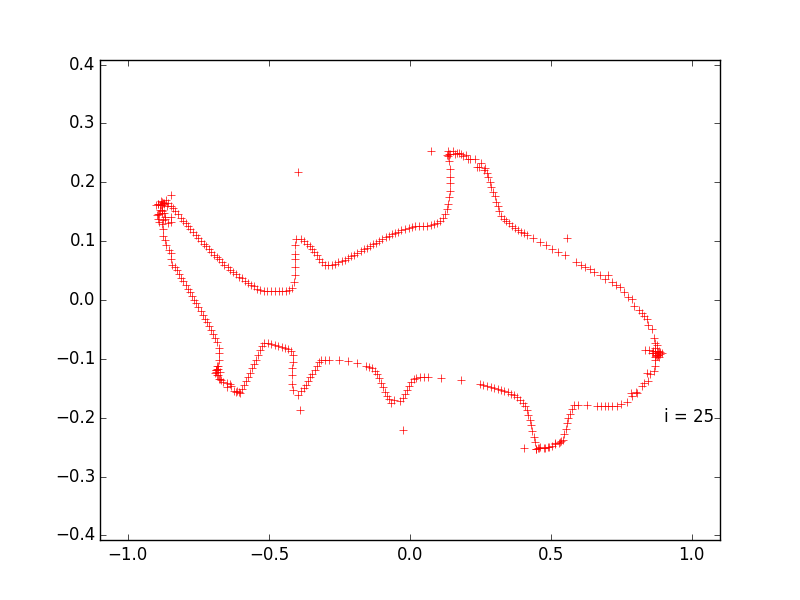
\includegraphics[scale=0.22]{2d/perimeter/shark-24}
    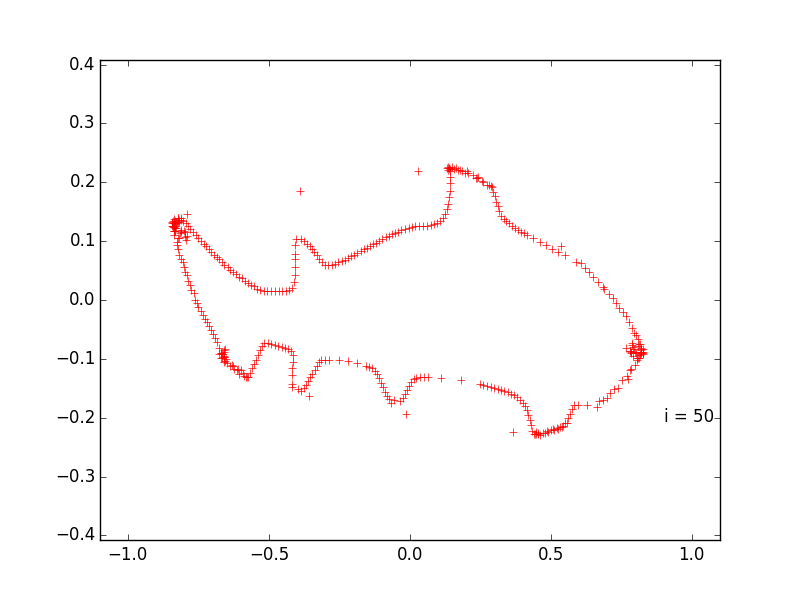
\includegraphics[scale=0.22]{2d/perimeter/shark-49}
    \subcaption{Perimeter flow of a shark: 0 / 25 / 50 iterations with a
        timestep of $ 0.05 $}

    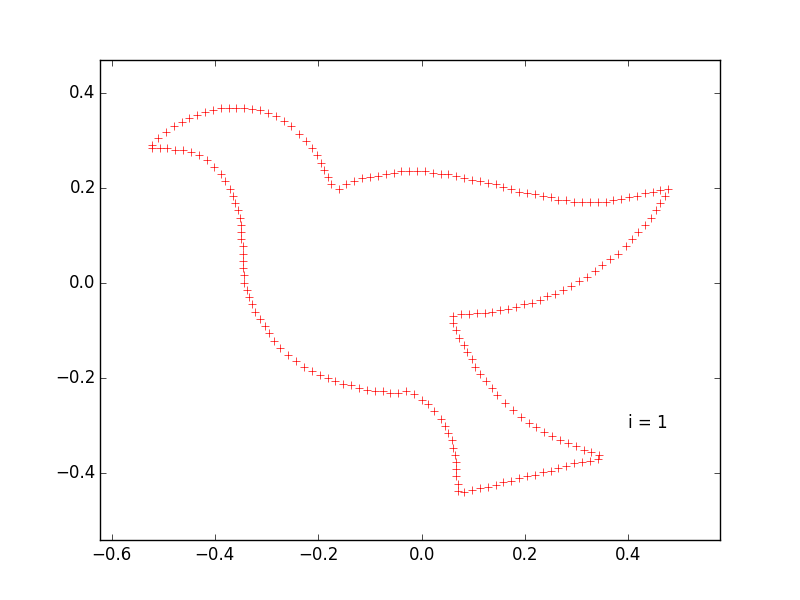
\includegraphics[scale=0.22]{2d/perimeter/bird-0}
    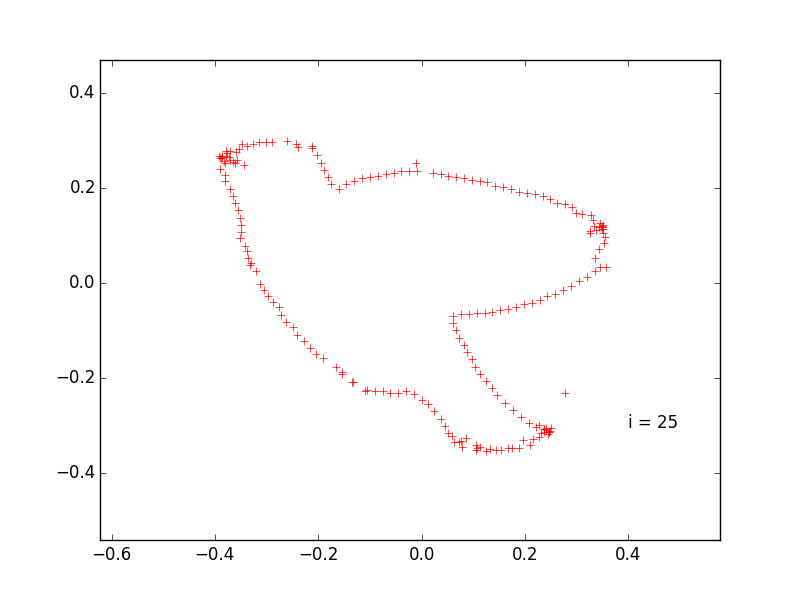
\includegraphics[scale=0.22]{2d/perimeter/bird-24}
    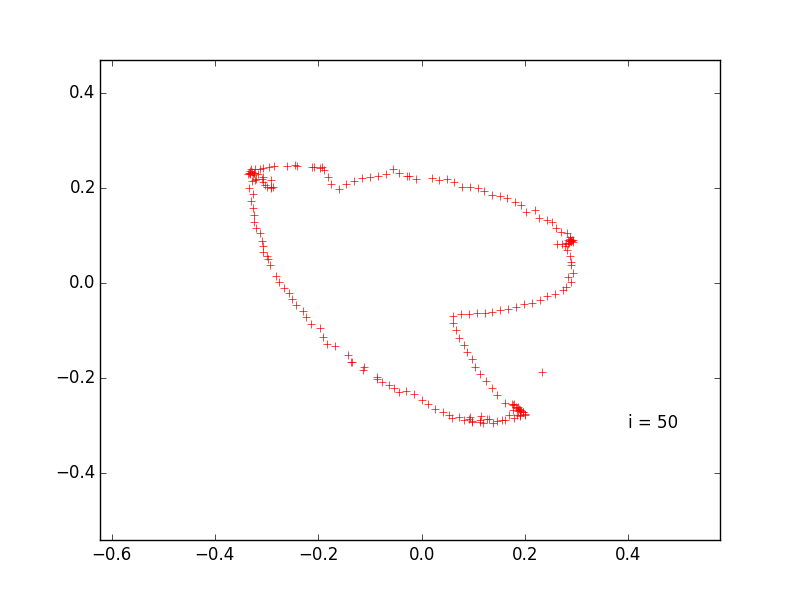
\includegraphics[scale=0.22]{2d/perimeter/bird-49}
    \subcaption{Perimeter flow of a bird: 0 / 25 / 50 iterations with a
        timestep of $ 0.05 $}
    \label{fig:shark_perimeter_flow}
\end{figure}

We test the smoothing property of our flow on points sampled on a square, see
the figure \ref{fig:area_perimeter_flow_square}. We can clearly see that our
discrete flow smooth the corners of the square.

\begin{figure}[h]
    \centering
    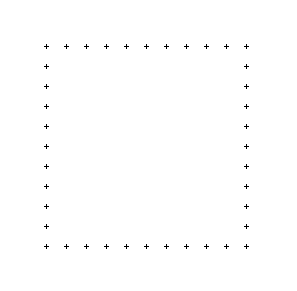
\includegraphics[scale=0.3]{2d/square-0}
    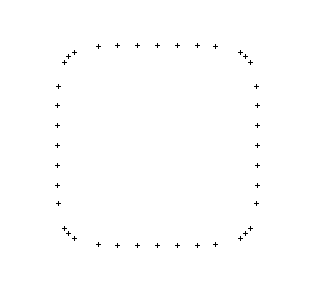
\includegraphics[scale=0.3]{2d/area/square-area-4-15-01}
    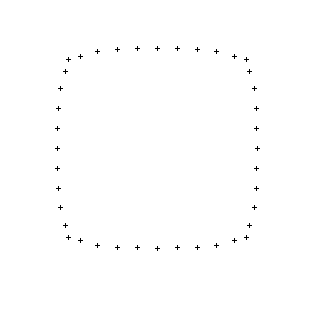
\includegraphics[scale=0.3]{2d/perimeter/square-perimeter-10-15-05}
    \caption{Area / perimeter flow on a square}
    \label{fig:area_perimeter_flow_square}
\end{figure}

We also verify that the area of the union of balls decreases with the number of
iterations, see the figure \ref{fig:area_time_decrease}.

\begin{figure}[h]
    \centering
    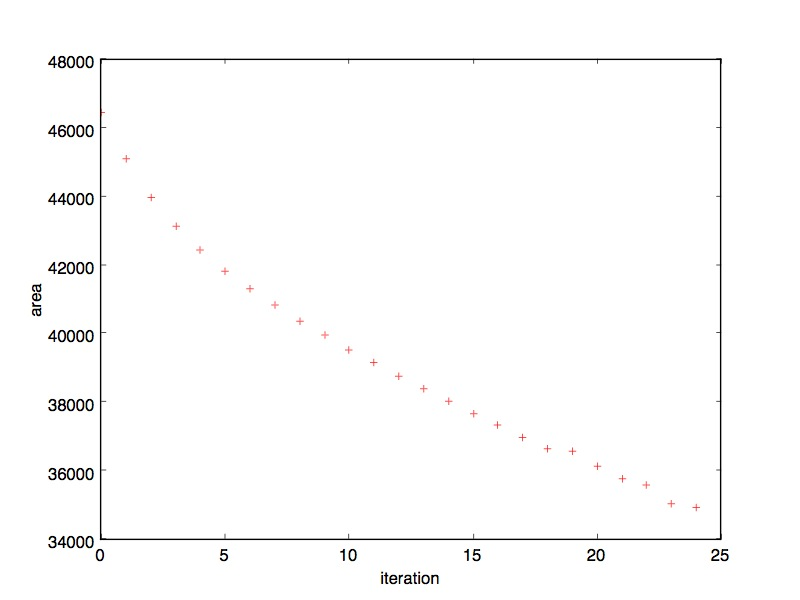
\includegraphics[scale=0.3]{2d/values-square-area}
    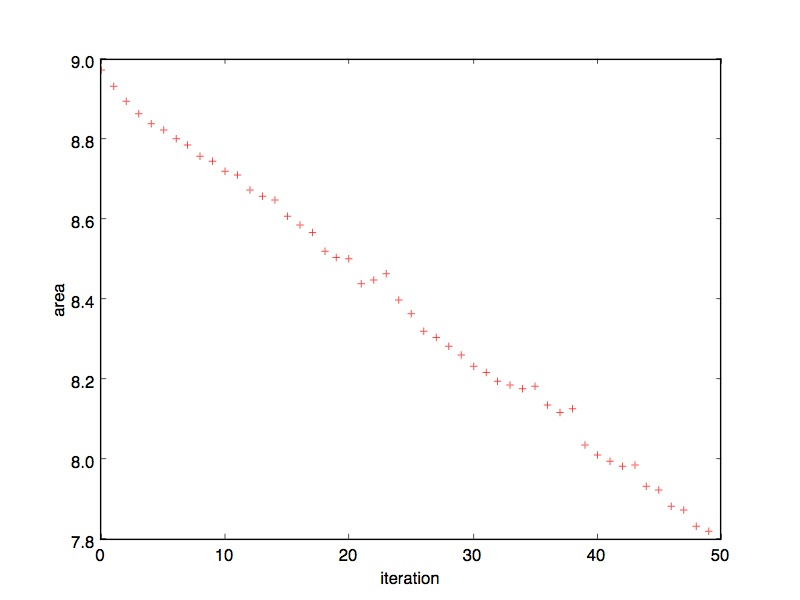
\includegraphics[scale=0.3]{2d/values-ellipse-perimeter}
    \caption{Evolution of the area on different point clouds with the area
        flow : square / ellipse}
    \label{fig:area_time_decrease}
\end{figure}

Next, we add some outliers around the ellipse and observe the effects of the two
flows: see the figures \ref{fig:ellipse_outliers_area_flow} and
\ref{fig:ellipse_outliers_perimeter_flow}. We see that the outliers are
"swallowed" by the initial point set in both cases. But, for the area flow, a
hole is created at the same place where the outliers were added.

\begin{figure}[h]
    \centering

    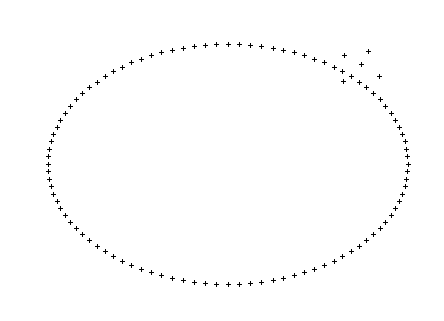
\includegraphics[scale=0.3]{2d/area/ellipse-100-01-15-outliers}
    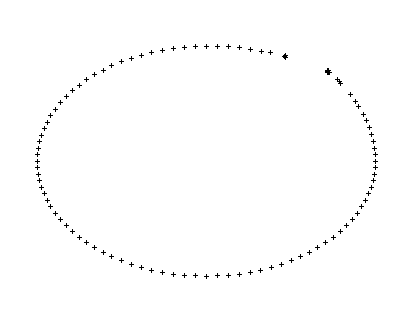
\includegraphics[scale=0.3]{2d/area/ellipse-100-01-15-outliers-40}
    \subcaption{Area flow of an ellipse with outliers: 0 / 40 iterations with a
        timestep of $ 0.1 $}
    \label{fig:ellipse_outliers_area_flow}

    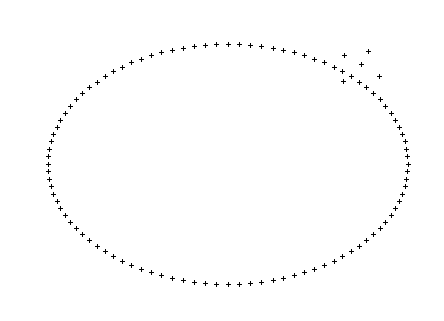
\includegraphics[scale=0.3]{2d/perimeter/ellipse-100-1-15-outliers}
    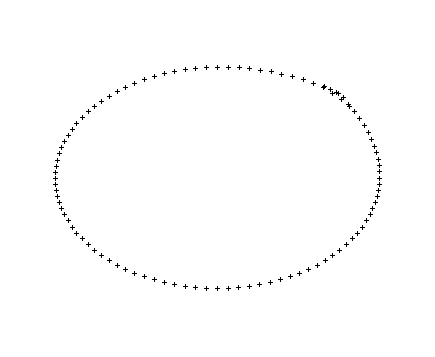
\includegraphics[scale=0.3]{2d/perimeter/ellipse-100-1-15-outliers-100}
    \subcaption{Perimeter flow of an ellipse with outliers: 0 / 100 iterations
        with a timestep of $ 1 $}
    \label{fig:ellipse_outliers_perimeter_flow}
\end{figure}

Then, we added some Gaussian noise on these points to test the robustness of our
algorithm, see the figures \ref{fig:ellipse_noise_area_flow} and
\ref{fig:ellipse_noise_perimeter_flow}.

\begin{figure}[h]
    \centering

    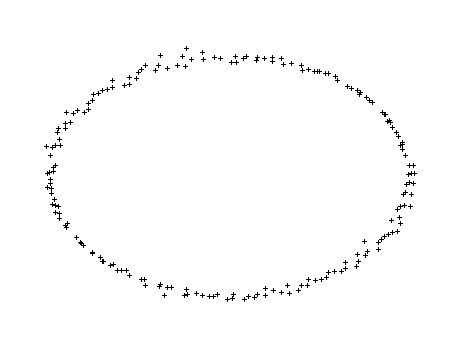
\includegraphics[scale=0.3]{2d/ellipse-noise-5-0}
    \includegraphics[scale=0.3]{2d/area/ellipse-noise-5-75}
    \subcaption{Area flow on a noised ellipse: 0 / 75 iterations with a timestep of $ 0.05 $}
    \label{fig:ellipse_noise_area_flow}

    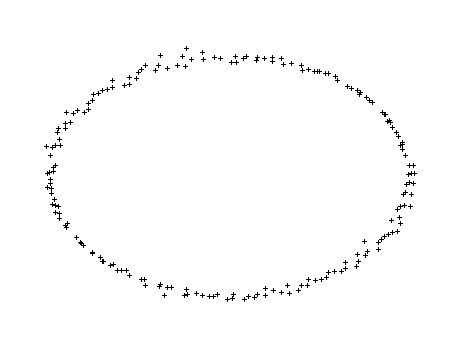
\includegraphics[scale=0.3]{2d/ellipse-noise-5-0}
    \includegraphics[scale=0.3]{2d/perimeter/ellipse-noise-5-75}
    \subcaption{Perimeter flow on a noised ellipse: 0 / 75 iterations with a timestep of $ 0.5 $}
    \label{fig:ellipse_noise_perimeter_flow}
\end{figure}

We notice that the gradient flow of the area may create holes in the point set
which is not the case for the gradient flow of the perimeter.

On the contrary, the gradient flow of the perimeter of the boundary will smooth
the point set while redistributing the points in an uniform way.

% TODO: explain why
This can be explained by looking on a simple case with two intersecting balls:
\begin{itemize}
    \item \textit{for the perimeter}: the gradients are directed towards the outside
        and so the balls will be merged because we can say, using the triangle
        inequality, that in order to minimize the perimeter the balls must come
        closer.
    \item \textit{for the area}: using the same reasoning, in order to minimize the area,
        it is possible that the gradients are oriented in opposite directions
        because the area gain may be more costly than moving the balls closer.
\end{itemize}

The chosen radius will also influence the smoothing: points which are too far
away from other points (at distance greater than the radius) will not move. The
more the radius is big, the more points will move in big groups. Indeed, the
radius indicates how to take the neighbours of a point into account, the more
neighbours we take into account the more "global" the movement will be.

We also add varying oscillations to our ellipse in order to see the
adaptive part of the algorithm. We generate oscillations with one or two
amplitudes.

For one constant amplitude, see the figures \ref{fig:ellipse_osc_perimeter_flow} and
\ref{fig:ellipse_osc_area_flow} and for two different amplitudes see
\ref{fig:ellipse_osc2_area_flow} and \ref{fig:ellipse_osc2_perimeter_flow}.

\begin{figure}[h]
    \centering

    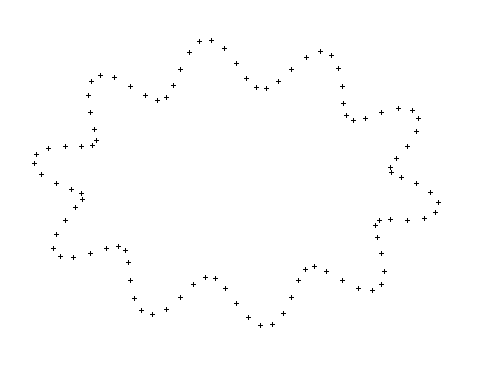
\includegraphics[scale=0.3]{2d/ellipse-osc-25-15-0}
    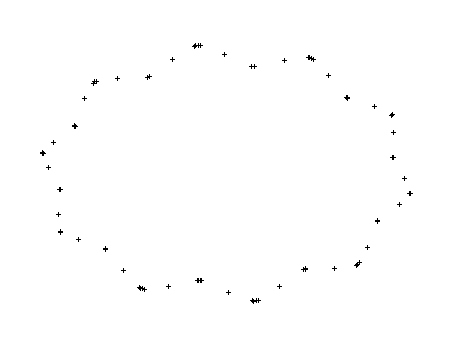
\includegraphics[scale=0.3]{2d/area/ellipse-osc-25-15-25}
    \subcaption{Area flow on an ellipse with oscillations (one amplitude) : 0 /
        25 iterations with a timestep of $ 0.05 $ and a radius of $ 15 $}
    \label{fig:ellipse_osc_area_flow}

    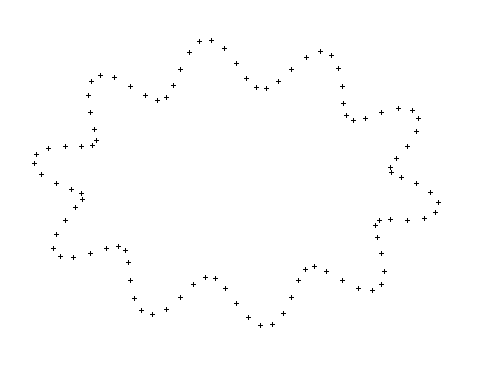
\includegraphics[scale=0.3]{2d/ellipse-osc-25-15-0}
    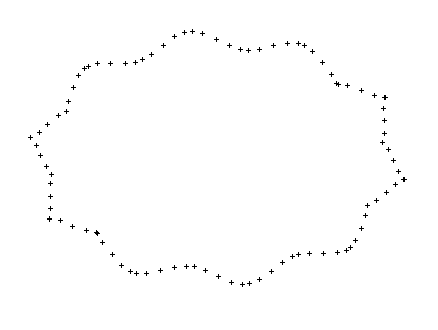
\includegraphics[scale=0.3]{2d/perimeter/ellipse-osc-25-15-50}
    \subcaption{Perimeter flow on an ellipse with oscillations (one amplitude):
        0 / 55 iterations with a timestep of $ 0.5 $ and a radius of $ 15 $}
    \label{fig:ellipse_osc_perimeter_flow}
\end{figure}

\begin{figure}[h]
    \centering

    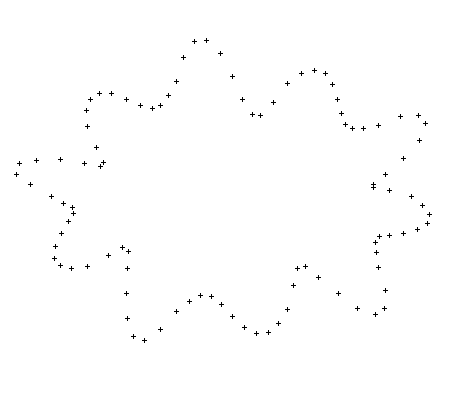
\includegraphics[scale=0.3]{2d/ellipse-osc2-20}
    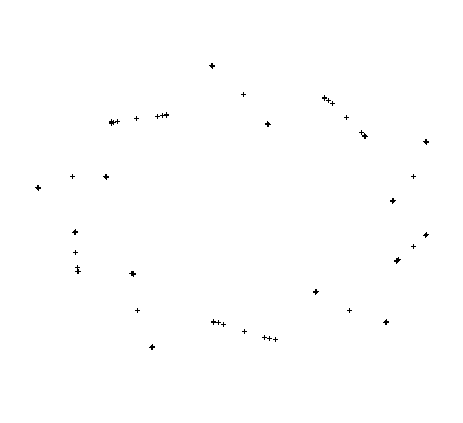
\includegraphics[scale=0.3]{2d/area/ellipse-osc2-20-15-25}
    \subcaption{Area flow on an ellipse with oscillations (two amplitudes): 0 /
        25 iterations with a timestep of $ 0.05 $ and a radius of $ 15 $}
    \label{fig:ellipse_osc2_area_flow}

    \includegraphics[scale=0.3]{2d/ellipse-osc2-20}
    \includegraphics[scale=0.3]{2d/perimeter/ellipse-osc2-20-15-55}
    \subcaption{Perimeter flow on an ellipse with oscillations (two amplitudes)
        : 0 / 55 iterations with a timestep of $ 0.5 $ and a radius of $ 15 $}
    \label{fig:ellipse_osc2_perimeter_flow}
\end{figure}

% TODO: explain why

Another experiment we did was to take points on a line segment and to fix its
endpoints. Then, we apply our flow on this point set. We expect the flow to
smooth the point set: points should get closer and closer to an uniformly
sampled set of points. See the figures \ref{fig:line_fixed_area} and
\ref{fig:line_fixed_perimeter} for the results.

\begin{figure}[h]
    \centering

    \includegraphics[scale=0.5]{2d/area/line-01-15-0}
    \includegraphics[scale=0.5]{2d/area/line-01-15-50}
    \subcaption{Area flow of points on a segment: 0 / 50 iterations with a timestep of $ 0.1 $}
    \label{fig:line_fixed_area}

    \includegraphics[scale=0.5]{2d/perimeter/line-05-15-0}
    \includegraphics[scale=0.5]{2d/perimeter/line-05-15-50}
    \subcaption{Perimeter flow of points on a segment: 0 / 50 iterations with a timestep of $ 0.5 $}
    \label{fig:line_fixed_perimeter}
\end{figure}

% TODO: explain why

In short, the two flows (area and perimeter of the boundary) have the following
common properties:
\begin{itemize}
    \item Smooth the point set: remove the outliers / noise
    \item Can be used to estimate the mean curvature
\end{itemize}

But, there are differences between the two flows. The main one is that the area
flow has the tendency to create holes in the point cloud. This difference is
removed when we use the weighted versions of the flows.

% {{{1 ASSESSMENT
\section{Assessment}

In this chapter, we saw how to simulate discrete mean curvature flows by using
the gradient of the volume of the $r$-offset of a point cloud.

The methods used in this chapter are hard to extend in 3D but have already been
done: see \cite{cazals2011computing}.

Also, we want to use polyhedral (anisotropic) norms, a thing that the previous
method does not allow since it only deals with intersection of a Voronoi cell
and a ball and we need a way to intersect a Voronoi cell and a polygon.

% TODO:
% - description
% - résultats
% - bilan + transition

% vim: set spelllang=en :
